\documentclass{article}[18pt]
\ProvidesPackage{format}
%Page setup
\usepackage[utf8]{inputenc}
\usepackage[margin=0.7in]{geometry}
\usepackage{parselines} 
\usepackage[english]{babel}
\usepackage{fancyhdr}
\usepackage{titlesec}
\hyphenpenalty=10000

\pagestyle{fancy}
\fancyhf{}
\rhead{Sam Robbins}
\rfoot{Page \thepage}

%Characters
\usepackage{amsmath}
\usepackage{amssymb}
\usepackage{gensymb}
\newcommand{\R}{\mathbb{R}}

%Diagrams
\usepackage{pgfplots}
\usepackage{graphicx}
\usepackage{tabularx}
\usepackage{relsize}
\pgfplotsset{width=10cm,compat=1.9}
\usepackage{float}

%Length Setting
\titlespacing\section{0pt}{14pt plus 4pt minus 2pt}{0pt plus 2pt minus 2pt}
\newlength\tindent
\setlength{\tindent}{\parindent}
\setlength{\parindent}{0pt}
\renewcommand{\indent}{\hspace*{\tindent}}

%Programming Font
\usepackage{courier}
\usepackage{listings}
\usepackage{pxfonts}

%Lists
\usepackage{enumerate}
\usepackage{enumitem}

% Networks Macro
\usepackage{tikz}


% Commands for files converted using pandoc
\providecommand{\tightlist}{%
	\setlength{\itemsep}{0pt}\setlength{\parskip}{0pt}}
\usepackage{hyperref}

% Get nice commands for floor and ceil
\usepackage{mathtools}
\DeclarePairedDelimiter{\ceil}{\lceil}{\rceil}
\DeclarePairedDelimiter{\floor}{\lfloor}{\rfloor}

% Allow itemize to go up to 20 levels deep (just change the number if you need more you madman)
\usepackage{enumitem}
\setlistdepth{20}
\renewlist{itemize}{itemize}{20}

% initially, use dots for all levels
\setlist[itemize]{label=$\cdot$}

% customize the first 3 levels
\setlist[itemize,1]{label=\textbullet}
\setlist[itemize,2]{label=--}
\setlist[itemize,3]{label=*}

% Definition and Important Stuff
% Important stuff
\usepackage[framemethod=TikZ]{mdframed}

\newcounter{theo}[section]\setcounter{theo}{0}
\renewcommand{\thetheo}{\arabic{section}.\arabic{theo}}
\newenvironment{important}[1][]{%
	\refstepcounter{theo}%
	\ifstrempty{#1}%
	{\mdfsetup{%
			frametitle={%
				\tikz[baseline=(current bounding box.east),outer sep=0pt]
				\node[anchor=east,rectangle,fill=red!50]
				{\strut Important};}}
	}%
	{\mdfsetup{%
			frametitle={%
				\tikz[baseline=(current bounding box.east),outer sep=0pt]
				\node[anchor=east,rectangle,fill=red!50]
				{\strut Important:~#1};}}%
	}%
	\mdfsetup{innertopmargin=10pt,linecolor=red!50,%
		linewidth=2pt,topline=true,%
		frametitleaboveskip=\dimexpr-\ht\strutbox\relax
	}
	\begin{mdframed}[]\relax%
		\centering
		}{\end{mdframed}}



\newcounter{lem}[section]\setcounter{lem}{0}
\renewcommand{\thelem}{\arabic{section}.\arabic{lem}}
\newenvironment{defin}[1][]{%
	\refstepcounter{lem}%
	\ifstrempty{#1}%
	{\mdfsetup{%
			frametitle={%
				\tikz[baseline=(current bounding box.east),outer sep=0pt]
				\node[anchor=east,rectangle,fill=blue!20]
				{\strut Definition};}}
	}%
	{\mdfsetup{%
			frametitle={%
				\tikz[baseline=(current bounding box.east),outer sep=0pt]
				\node[anchor=east,rectangle,fill=blue!20]
				{\strut Definition:~#1};}}%
	}%
	\mdfsetup{innertopmargin=10pt,linecolor=blue!20,%
		linewidth=2pt,topline=true,%
		frametitleaboveskip=\dimexpr-\ht\strutbox\relax
	}
	\begin{mdframed}[]\relax%
		\centering
		}{\end{mdframed}}
\lhead{New Venture Creation}


\begin{document}
\begin{center}
\underline{\huge New Venture Creation - Paul Burns}
\end{center}
\section{The New Venture Creation Framework}
In recent times there has been a high degree of volatility in global markets, this may be caused by the increased interconnectivity brought by the internet. In highly connected systems small changes tend to be amplified. Actions in one part of a market can have unexpected and rapid consequences on another part of it.\\
\\
Change has become a continuous process which large firms have difficulty dealing with, whereas small ventures are able to find opportunities in.\\
\\
\textbf{Intrapreneurs} - People within a large organisation who create new ventures, while remaining under salaried employment, and all risk goes to the employers\\
\textbf{Social/Civic Entrepreneurs} - People who are willing to invest their own time and risk their own capital for little or no financial return.\\
\textbf{Entrepreneurs} - Create and/or exploit change for profit\\
\textbf{Salary-Substitute Firms} - Firms that generate an income comparable to what someone might earn as an employee\\
\textbf{Lifestyle Firms} - Firms that allow someone to pursue a particular lifestyle whilst enabling them to earn an acceptable living\\
\textbf{Entrepreneurial Firms} - Firms that bring innovative ideas and ways of doing things to the market
\subsection{Barriers and triggers to entrepreneurship}
Barriers:
\begin{itemize}
\item Need for regular income
\item Lack of start up capital
\item Lack of self belief
\item Fear of loss of capital
\item Risk aversion
\end{itemize}
Triggers:
\begin{itemize}
\item Made redundant
\item They have no alternative
\item Yearn for independence and recognition of their achievements
\item The prospect of becoming rich
\item Wanting increased personal development
\end{itemize}
\subsection{New Venture Creation}
Things needed to create a new venture:
\subsubsection{Personal character traits that incline you towards entrepreneurship}
Not everyone is well suited to self employment, some people can't handle the stresses it produced or enjoy the challenges it presents
\subsubsection{A good business idea}
\subsubsection{The necessary skills to deliver your product/service idea}
Training provides knowledge of how the sector works and a network of contacts who could become customers or suppliers. It also helps learn these things and make mistakes at somebody else's expense. 
\subsubsection{A plan to launch and grow your business}
The act of planning helps you prepare for uncertainties and gives you the frameworks that make you better react to unexpected threats and opportunities
\subsubsection{The resources you need to launch and grow your business}
You need to minimise the resources you need and assess how much and what sort of finance to look for. The business plan will help you attract that finance
\subsection{Business Planning}
The Principles of Planning:
\begin{itemize}
\item \textbf{Know where you are} - Understand strengths and weaknesses, the skills you bring, resources you can mobilise and if you have what it takes to be and entrepreneur
\item \textbf{Know where you want to go} - Have a clear idea of the business opportunity and what you want your business to become in the future
\item \textbf{Plan how to get there} - Plan how to make this happen, how to get customers, combat competition and lead staff
\end{itemize}
Planning needs to be a continuous process as there is a high degree of uncertainty in a new venture. Planning helps to estimate the resources required.
\subsection{The New Venture Creation Framework}
\begin{center}
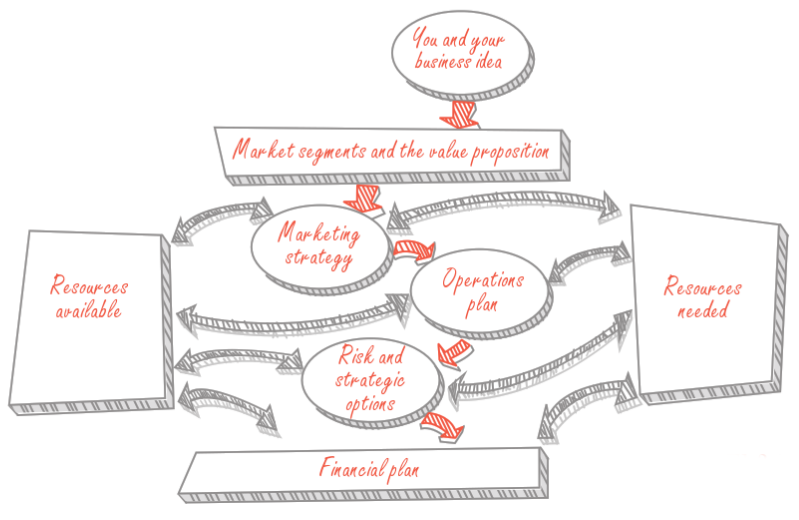
\includegraphics[width=12cm]{nvc.png}
\end{center}
\subsubsection{You and your business idea}
If you have the personal characteristics to be an entrepreneur and if your characteristics match your venture. A good business model describes how you will go about delivering your business idea to customers. Even if the business idea has merit, without the business plan you do not have a viable business. You also need marketing, operations and financial plans based on the resources you need and have. You need to identify and minimise the risks you take
\subsubsection{Market segments and the value proposition}
At the core of a business model is the identification of different groupings of customers with similar characteristics - called \textbf{market segments}. The motivations each segment has for buying your product or service are the \textbf{benefits} they are seeking. Pulling these benefits together for each segment is called your \textbf{value proposition}. Before you develop this you need to understand the structure of the market and industry you are entering and the value propositions they are offering customers.
\subsubsection{Marketing Strategy}
This describes how you will deliver your value proposition to each of the identified customer segments. The tool for delivering this is called the \textbf{marketing mix} - price, promotion/communication, service etc. A good marketing strategy helps you develop \textbf{competitive advantage} against other companies in your market. This needs to cover launch, core and growth strategies.
\subsubsection{Operations plan}
This highlights the practical things you need to do to launch a new venture. These range from legal to operating issues, including \textbf{partnership} opportunities. It should identify those key activities you need to undertake to ensure success .
\subsubsection{Risk and strategic options}
The business model should show the major risks and how they might be mitigated or avoided. It should identify the \textbf{critical success factors} that underpin the operations of the business and recognise different ways of doing things if an obstacle is met, called \textbf{strategic options}.
\subsubsection{Resources available and needed}
This defines the resources you bring to the business, \textbf{human, social, intellectual and financial}, and the resources you need. A major component of this is your ability to pull together and lead a management team
\subsubsection{Financial plan}
This shows the \textbf{profit} the business should generate and how it is used. It shows the \textbf{cash flow} of the business and the external finance that will be required. It is a set of \textbf{financial forecasts} - revenues, related costs and resulting financial structures of the business
\subsection{The Business Model Canvas}
\begin{center}
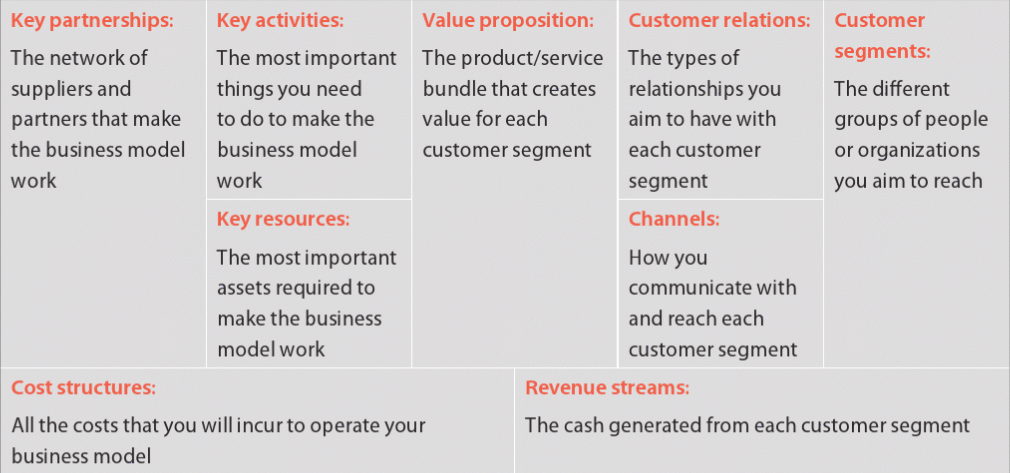
\includegraphics[width=12cm]{business_model_canvas.png}\\
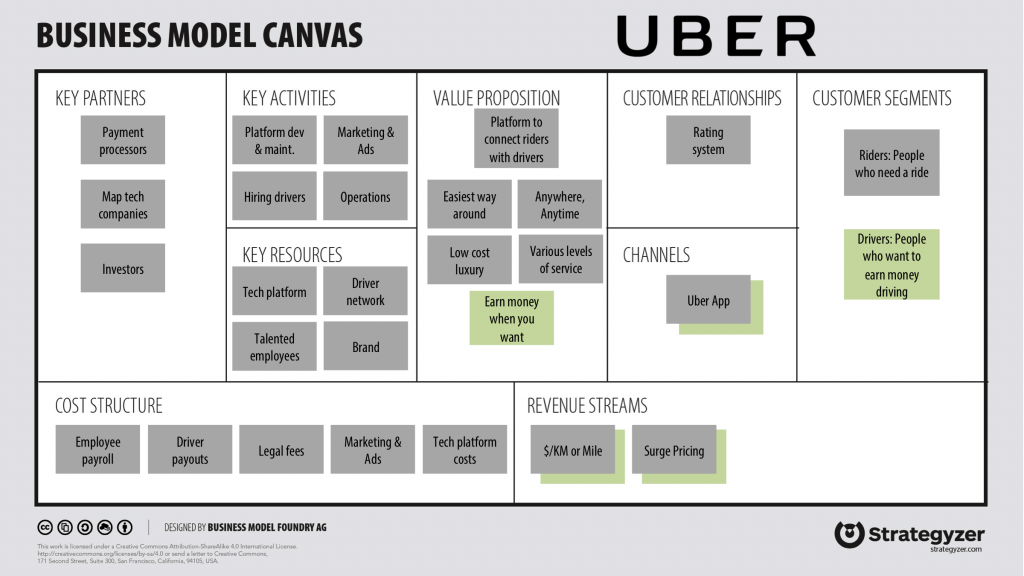
\includegraphics[width=12cm]{uber_canvas.png}
\end{center}
The left side of the canvas is driven by efficiency and the right side is driven by value to customers\\
\\
\subsection{The Business Plan}
The Business Plan is a document that sets out your business idea and the business model upon which it is based.\\
\\
The advantage of developing a business plan using the New Venture Creation Framework is that it forces you to think systematically and in detail about the future of the business. It forces you to think through the options that are open to you and justify the decisions you take, whilst thinking through the consequences of your actions.








\end{document}